\label{sec:RESULTS}

This following section aims to explain the thermo-electromagnetic phenomena underlying the simulation. Turns out, when considering the proper symmetries the simulations can be reduced in computation significantly \footnote{One of the critical success criteria.}.
\\

In the context of a straight cylindrical copper wire that carries a alternating current at standard frequencies, we consider the values at the tables to obtain $\epsilon = 1.4765 * 10^{-6}$, with
\begin{equation}
    w_p = \frac{nq^2}{\epsilon_0 m} = 1.645* 10^{16} [\frac{C^2 \Omega}{ m^2 s kg}],
\end{equation}
being the plasma frequency. Recall this frequency is used to calculate $\epsilon $ from Drude's dielectric function summarized by equation (9).
\\
Most importantly we must check quasi-magnetostatic conditions are met. Submitting our values to the conditions stated in equations \ref{eq:MaxwellQuasiMagnetostatic}, we obtain
\begin{equation*}
    \frac{j_D}{j_{ext}} =  \mu\epsilon w  R^2 = 2.1*10^{-11} << 1
\end{equation*}
when one considers no external currents, this condition is instantly met. For the latter and most important condition, we have
\begin{equation*}
     \frac{j_D}{j_{f}} = \frac{\epsilon w}{\sigma} = w \tau_E = \frac{\epsilon(w_p)*w}{\sigma}= 9.3*10^{-12} << 1,
\end{equation*}
in the code (annex 1) is found as \textsc{condition 2} and it is calculated with the values in the table in section II. \\

With both conditions met, it is secure to adopt the quasi-magnetostatic approximation with an accuracy of 99 percent. Furthermore, \cite{zangwill2013modern} shows that it is possible to derive the wave equation that governs the cable from Maxwell equations in the quasi-magnetostatic approximation \ref{eq:MaxwellQuasiMagnetostatic} obtaining:
\begin{equation}
    \nabla ^2 E =  \mu \sigma \frac{\partial E}{\partial t}.
\end{equation}

Assuming AC harmonic current $I(t)=I_0 e^{-iwt}$ allow us to propose the following anzatz $\xi(r,t)=E(r) \Psi(t)$. Furthermore, analysis in cylindrical coordinates $(\rho,\theta,z)$ has two symmetries in $\theta$ and $z$ that we'll exploit. This gives rise to a second-order ordinary differently equation describing the electromagnetic fields inside the cable 
\begin{equation}
\label{eq:diff-eqq-cylindrical}
    \rho \frac{\partial}{\partial \rho} (\rho \frac{\partial E}{\partial \rho}) + \kappa^2 \rho^2 E = 0 .
\end{equation}
Where the variable $\kappa = \sqrt{i\mu\sigma w} = (1+i)/\delta$ is closely related to the skin depth. Moreover, solutions to the former differential have the Bessel functions: $J_0(\kappa\rho)$ and $J_1(\kappa\rho)$; Related by Ampere-Maxwell in equation \ref{eq:MaxwellQuasiMagnetostatic}. Numerical field simulation can be implemented in the two dimensional transversal cut and dependent only on the radial variable $\rho$. If the cable is oriented in the $z$ direction, it is possible to define the fields
\begin{equation}
    E(\rho, t) = \Vec{z}  A J_0(\kappa \rho) exp(-iwt),
\end{equation}
and
\begin{equation}
    B(\rho, t) =  \Vec{\theta} \hspace{ 0.1cm} \frac{\kappa \rho}{iw} J_1(\kappa \rho) exp(-iwt).
\end{equation}
\\
Visualizing the behavior of the latter expressions we obtain the following figure
\begin{figure}[H]
    \centering
    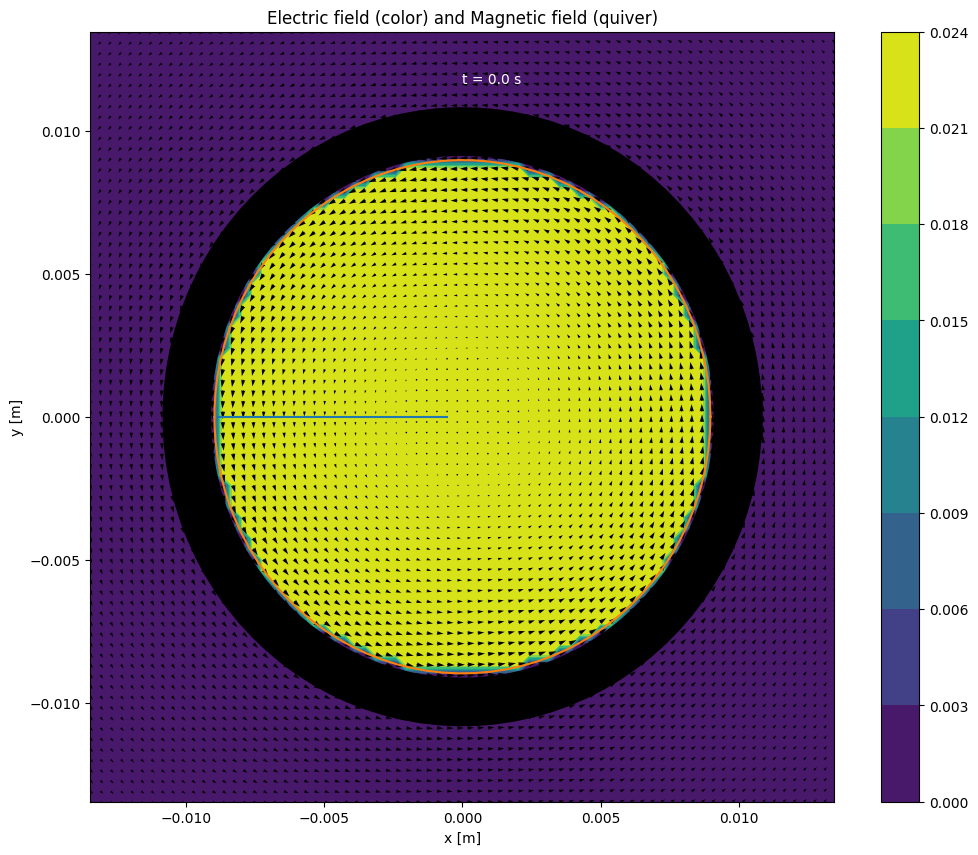
\includegraphics[scale=0.35]{Figures/em-fields-cable.png}
    \caption{Electromagnetic Field Visualization. Color represents electric field intensity and the quiver represents the magnetic field.}
    \label{fig:emfields-colorquiver}
\end{figure}

Furthermore, analyzing the behavior with respect to the radial distance we observe that the electric field has stronger values in the surface, explaining the skin effect. The magnetic field is also interesting because it illustrates the boundary conditions relating the inner and outer fields. 
\begin{figure}[H]
    \centering
    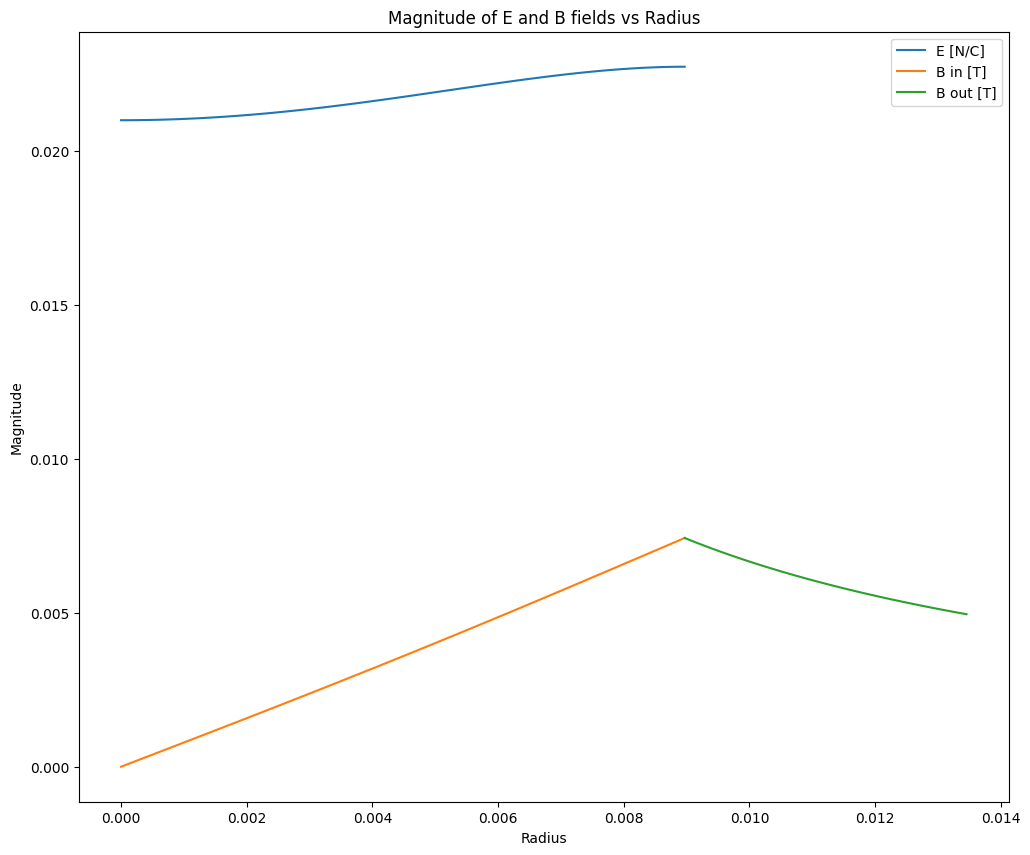
\includegraphics[scale=0.35]{Figures/magnitude-EvsB-radius.png}
    \caption{Electromagnetic fields as a function of radius.}
    \label{fig:emfields-radius}
\end{figure}

\subsection{The physics explaining the energy of the fields}
With these fields you can take two alternatives to calculate energy dissipation with poynting's vector and with the work energy of the electron-field interaction \footnote{Recall from such analysis, Joule´s rule was derived.}. The work proceeds to analyze the former and then the latter. 
\\
Poynting's vector is defined by Jackson \cite{jackson1999classical} as
\begin{equation}
    S = \frac{1}{\mu} E \times B \hspace{0.2cm} [\frac{J}{m^2s}].
\end{equation}
Particularly, we are interested on this vectors value at the surface since the flux of energy as heat is happening at the surface of the cable. The power $P = S* A$ is related to the heat energy $Q = P*t$, where area is determined by the cable parameters and the time is a single period of the AC oscillation. The results are presented in the figures bellow
\begin{figure}[H]
    \centering
    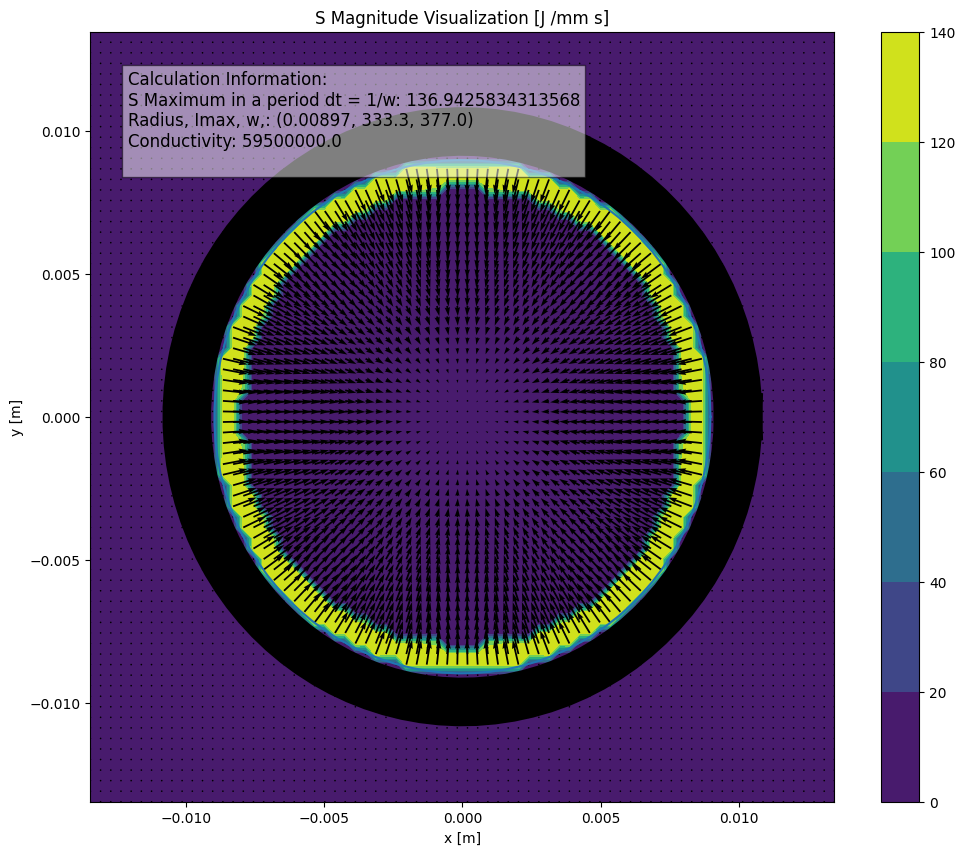
\includegraphics[scale=0.35]{Figures/poyinting-vector-cable.png}
    \caption{Poynting's Vector Visualization}
    \label{fig:poynting-colorquiver}
\end{figure}

For practical purposes, it is only necessary to arrive at Poynting's vector value. In fact, thermal simulation software calculate temperature distribution in a system given this value. For example, SolidWorks (R) only asks for poyntings value over the surface of the cable to calculate temperature. This reduces computation because in the case of more advanced software like ANSYS, the computer needs to solve Maxwells equations in all space and then solve the thermal or mechanical equations using finite element analysis. This work shows that is it possible to reduce the fist step of computation.
\\
For the sake of completeness, we present the power calculations in the following figure.
\begin{figure}[H]
    \centering
    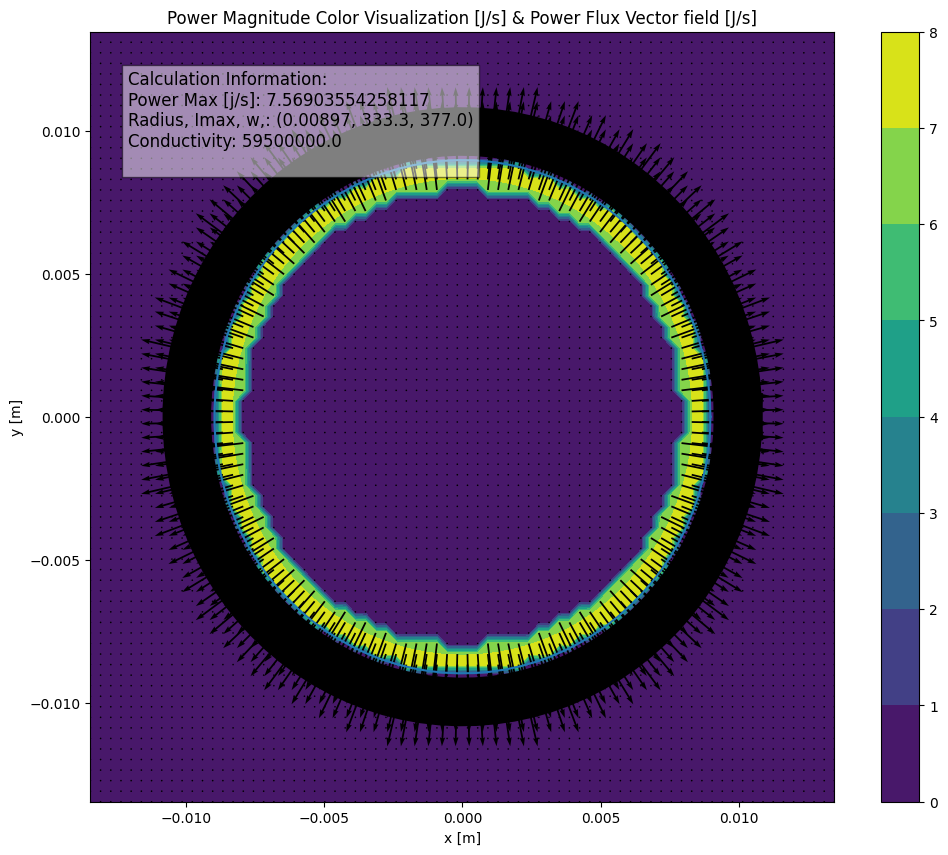
\includegraphics[scale=0.35]{Figures/power-q-cable.png}
    \caption{Power Visualization}
    \label{fig:power-colorquiver}
\end{figure}
As shown, the maximum power in purely electromagnetic calculations is 7.569 [W] while a the quick formula for Joule's rule yields 7.386 [W]. This difference can be explained due to the nature of both calculations. However, according to the modern theory of electrodynamics the power is greater than Joule's rule simplification. Therefore, using Joules rule can lead to problems because it gives lower heat fluxes than theory predicts.

\subsection{Skin effect}
Equation \ref{eq:diff-eqq-cylindrical} is related to the induction condition expressed in \ref{eq:inductioncondition} leading to the understanding how skin depth relates to induction via: $B_F/B_ext = \mu \sigma w R^2 = 2*R^2 / \delta^2$. Evaluating this condition in the system proposed we have $2.226 > 1$. The result hints at the fact that small induction will be present on our system. Moreover, relationship introduced above yields an expression for the skin depth of the form
\begin{equation}
    \delta(w) = \sqrt{\frac{2 }{\mu \sigma w}}.
\end{equation}
The former equation is the distance in meters from the surface into the core of the cable shown in figure \ref{fig:emfields-colorquiver}. The value obtained for the system under study is $\delta(w) = 0.00842$; just below the value of the nuclei radius $R$. This value is expected because condition \ref{eq:inductioncondition} expects small inductions.

\subsection{The physics underlying Joule's rule}
Notice that when considering Ohmic matter $j = \sigma E$ we can easily visualize the current density. Obtaining the current distribution is of great importance in order to validate our results. To understand why, we need to dive into the thermodynamics of the problem. \\
\begin{figure}[H]
    \centering
    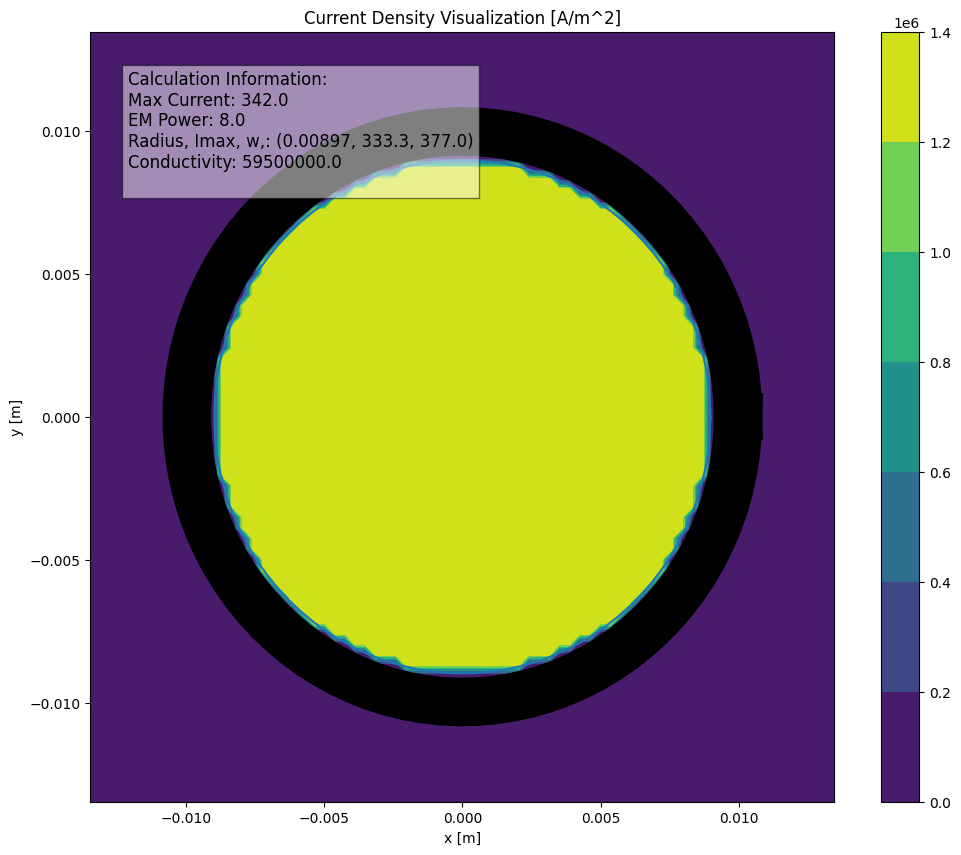
\includegraphics[scale=0.35]{Figures/current-density-cable.png}
    \caption{Current density Visualization}
    \label{fig:current-color}
\end{figure}
\begin{figure}[H]
    \centering
    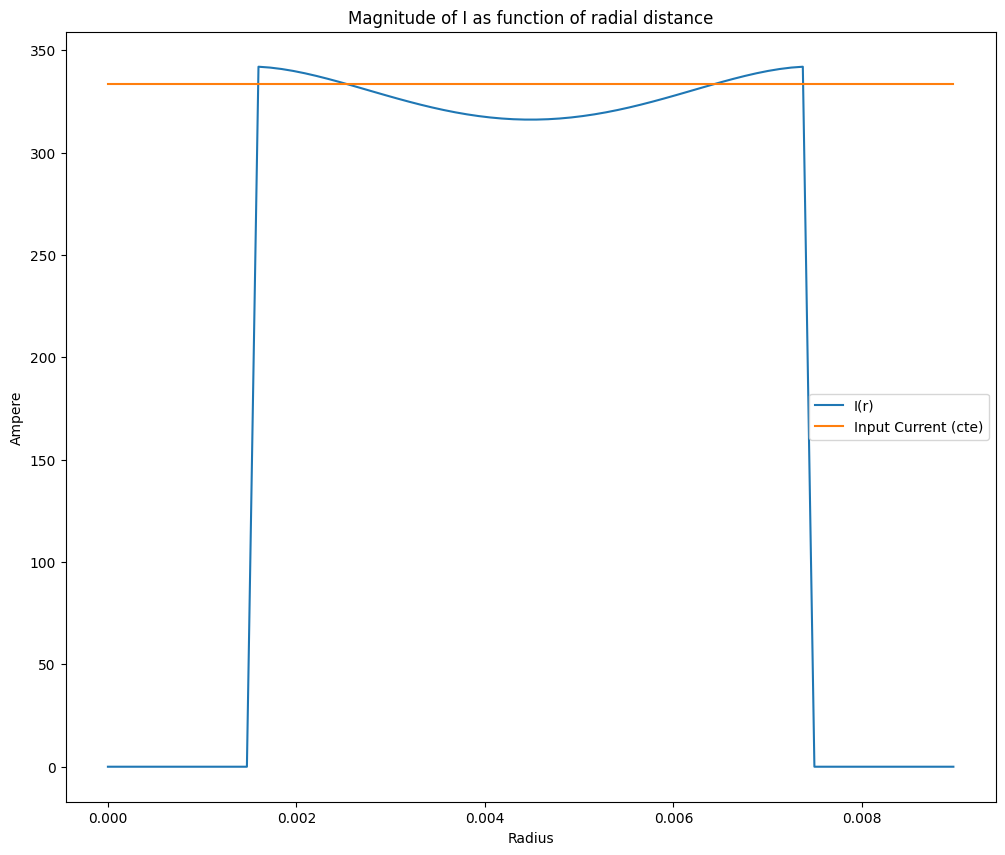
\includegraphics[scale=0.35]{Figures/magnitude-current-radius.png}
    \caption{Current Magnitude as a function of radius}
    \label{fig:current-color}
\end{figure}


Recall the first law of thermodynamics in a conservative system involving the cable and the air of the exterior. Energy must be conserved, thus $Q=W$ and for our cable model we have
\begin{equation}
    dQ/dt = \int d^3r \nabla \cdot (j(\rho)*\phi(t)) ,
\end{equation}
this will give the energy loss considering the work made by the E field \footnote{Recall magnetic fields don't make work.} on the electrons inside the cable. The volumetric evaluation of this integral yields an average value of 7.56 $[W]$. Which agrees with electromagnetic calculations. 

%\subsection{Forces on Cables}
%% Calcular fuerzas entre 3 cables en condiciones de corto circuito

